\documentclass[conference]{IEEEtran}
\IEEEoverridecommandlockouts
% The preceding line is only needed to identify funding in the first footnote. If that is unneeded, please comment it out.
\usepackage{cite}
\usepackage{amsmath,amssymb,amsfonts}
\usepackage{algorithmic}
\usepackage{graphicx}
\usepackage{textcomp}
\usepackage{xcolor}
\def\BibTeX{{\rm B\kern-.05em{\sc i\kern-.025em b}\kern-.08em
T\kern-.1667em\lower.7ex\hbox{E}\kern-.125emX}}
\begin{document}

\title{Optimizing Illumination: Using an Evolutionary Algorithm to Balance Artificial and Natural Light in Rooms
}

\author{
    \IEEEauthorblockN{Ali Asghar Chakera}
    \IEEEauthorblockA{\textit{Department of Computer Science} \\
        \textit{Habib University}\\
        Karachi, Pakistan \\
        0009-0007-2038-9139}
    \and
    \IEEEauthorblockN{Hafsa Khurram}
    \IEEEauthorblockA{\textit{Department of Computer Science} \\
        \textit{Habib University}\\
        Karachi, Pakistan \\
        0009-0006-1400-2148}
    \and
    \IEEEauthorblockN{Syed Ibrahim Ali Haider}
    \IEEEauthorblockA{\textit{Department of Computer Science} \\
        \textit{Habib University}\\
        Karachi, Pakistan \\
        0009-0000-2714-992X} 
    \and
    \IEEEauthorblockN{Syeda Saleha Raza}
    \IEEEauthorblockA{\textit{Department of Computer Science} \\
        \textit{Habib University}\\
        Karachi, Pakistan \\
        saleha.raza@sse.habib.edu.pk}
}

\maketitle

\begin{abstract}
    This report describes the application of Computational Intelligence (CI) techniques to optimize the number of artificial light sources in a physical space while taking into account the presence of external light sources, such as sunlight. The project aims to reduce electricity consumption through artificial light sources, which can account for up to 15\% of the average electricity bill. The approach involves the use of evolutionary algorithms to simulate the process of natural selection and finds the optimal number and placement of artificial light sources in the room. The fitness of each solution will be evaluated based on an objective function that considers factors such as the number of lights, natural sources of light, obstacles in the room, shadows, and light intensity threshold for the entire room. The report also outlines the realistic constraints used in the project, including specific calculations for sunlight entering the room, and the physical space data set, which contains information such as the number and position of walls and windows. Relevant work in the area is discussed, including the importance of incorporating natural light sources and the use of genetic algorithms in similar projects. The proposed solution aims to provide a cost-effective and environmentally friendly way of optimizing lighting in physical spaces.\\
\end{abstract}

\begin{IEEEkeywords}
    Evolutionary Algorithm, Computational Intelligence, Artificial Light Optimization
\end{IEEEkeywords}

\section{Introduction}

For the scope of this project, we created a room that contains tiles,
windows, obstacles, windows (for sunlight), shadows, and artificial lights. All five of these elements contributed to the final
fitness function that is used. For this project, we have divided the room into
100 tiles with \(10*10\) dimensions, however for future work this can be easily customized given any dimensions.

\subsection{Motivation and related work}
The problem of \textit{Optimizing Artificial Lighting in a room} has been addressed in a
number of papers. In \cite{icict_2019}, the authors use a genetic algorithm to
optimize the number of lights in a room. The fitness function used in the paper
considers the number of lights and the light intensity threshold for the entire
room. The authors also consider the position of the lights in the room and
their distance from the walls. The paper does not take into account the
presence of natural light sources, such as sunlight, shadows, and the position of the
windows in the room. Our paper is an extension of the same problem with the
added constraint of natural light. The motivation behind this paper is to
reduce the electricity consumption of a room by optimizing the number of
artificial lights in the room. This is done by taking into account the presence
of natural light sources, such as sunlight, and the position of the windows in
the room. This paper aims to provide a cost-effective and environmentally
friendly way of optimizing lighting in physical spaces.

\section{Technical Background}
Genetic algorithms are a type of optimization algorithm,
meaning they are used to find the optimal solution(s) to a
given computational problem that maximizes or minimizes a
particular function. Genetic algorithms represent one branch of
the field of study called evolutionary computation, in which
they imitate the biological processes of reproduction and
natural selection to solve for the ’fittest’ solutions \cite{ref9}. Like in
evolution, many of a genetic algorithms processes are random,
however, this optimization technique allows one to set the level
of randomization and the level of control \cite{ref9}. During each
generation, three basic genetic operators are applied to each
chromosome with certain probabilities, i.e. selection, crossover
and mutation \cite{ref9}.
\subsection{Procedure}
The general procedure for Genetic Algorithms, as described by \cite{ref9}:\\
\begin{enumerate}
    \item  \textbf{Start:} Generate random population of n chromosomes
(suitable solutions for the problem).
    \item \textbf{Fitness:} Evaluate the fitness f(x) of each chromosome x
in the population.
    \item \textbf{New Population:} Create a new population by repeating
following steps until the new population is complete.
    \begin{enumerate}
        \item \textbf{Selection:} Select two parent chromosomes from a
        population according to their fitness (the better fitness,
        the bigger chance to be selected).
        \item \textbf{Crossover:} With a crossover probability cross over the parents to form a new offspring (children). If no
        crossover was performed, the offspring is an exact copy of the parents.
        \item \textbf{Mutation:} With a mutation probability mutate new offspring at each locus (position in chromosome).
        \item \textbf{Accepting:} Place new offspring in a new population.
    \end{enumerate}
    \item \textbf{Replace:} Use newly generated population for a further run of the algorithm.
    \item \textbf{Test:} If the end condition is satisfied, stop, and return the best solution in the current population.
6) Loop: Go to step 2.
\end{enumerate}
\section{Problem Description}
\subsection{Tiles}

\subsubsection{Initialisation}

% The IEEEtran class file is used to format your paper and style the text. All margins, 
% column widths, line spaces, and text fonts are prescribed; please do not 
% alter them. You may note peculiarities. For example, the head margin
% measures proportionately more than is customary. This measurement 
% and others are deliberate, using specifications that anticipate your paper 
% as one part of the entire proceedings, and not as an independent document. 
% Please do not revise any of the current designations.

The Tiles in the Room class were initialized at the standard grid of $10 \times 10$. The
length and width of the grids were initialized by the following formulas and
these were used throughout for the purpose of calculations etc.
\begin{equation}
    Width_{Tile} = Width_{Room}/10
\end{equation}
\begin{equation}
    Length_{Tile} = Length_{Room}/10
\end{equation}

Each Tile is also initialized to be completely empty in terms of light. Light
in each Tile is stored in three different areas for different kinds of
lighting.\\

\subsubsection{Lit}
This is a variable that stores a boolean value which turns to True if the Tile is lit at either minimum capacity or minimum fill. Both of these are calculated in the Room function. This is one of the most important variables since this is what we count at the count lit tiles function. \\

\subsubsection{Fill vessel}
Since Light from a light bulb or LED spreads in a circle shape it is possible for a tile to be lit from either of the eight sides that the tile has. This is why each tile has a list with 8 positions that stores its fill from each side. This fill is calculated in the Room's lit tiles function. With this paper, we set the minimum fill at 0.6 ie 60\% of the total Tile's area. If the area of the tile exceeds this area we will mark Lit as True. 

\begin{figure}
    \centering
    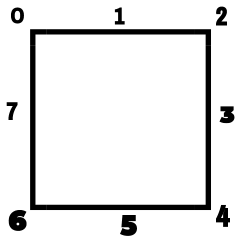
\includegraphics{Untitled design (2).png}
    \caption{Representations of the directions}
    \label{fig:fill_vessel}
\end{figure}
\subsubsection{Intensity}
Lit is also dispersed around the room in different forms where it may not be as intense as direct light. What we see in such circumstances is that the light is dispersed around with decreasing intensity as the distance between the area or in this case the tile increases. To store such irregular amounts we use the intensity variable where again if the intensity crosses minimum intensity the area is marked as lit. 
\subsection{Lights}
The lights class is a straightforward class that can be initialized with its position on the grid and the height of the ceiling ie. the height at which it is placed. For this paper, we assume that the height of the ceiling and that of the Lights is the same. Along with this we can return the length and the starting position of the circle of direct light that the light produces. Each light has something called the beam angle which is basically the limit till which the light is formed. % add citation here
The light spread is calculated according to this angle. 
\begin{figure}
    \centering
    \includegraphics{beam angle.png}
    \caption{Beam Angle Visualisation}
    \label{fig:fill_vessel}
\end{figure}

This angle is calculated by the following equation:
\begin{equation*}
    spread = height \cdot tan(beam\ angle)
\end{equation*}
This spread and the center of the circle are returned to the Room class for its calculations. 
\subsection{Windows}
The windows in the room can be placed at any of the four sides of the room.
They are defined as follows:
\begin{itemize}
    \item $Direction = \{North, South, East, West\}$
    \item $Starting Point = \{x, y\}$ either $x$ or $y$ is 0 or the max width or length respectively depending on the direction of the window
    \item $Length = l$
    \item $Width = w$
    \item $Height = h$ (height from the floor)
\end{itemize}
We calculate the area of the direct sunlight region in the room with the help of the \textit{Sun's} altitude $Sun_{altitude}$ at different times of the day which we obtained from \texttt{ephem} \cite{ephem}.\\

This altitude is used to calculate the spread of natural light in the room for these calculations we make the following assumptions. 
\begin{itemize}
    \item The sun is always above the window at all times that the sun is out
    \item That the sun is always in front of the window ie at a \(90\deg\) angle at the window. 
    \item That the direct sunlight entering the room will always be greater than the light from the lights. 
\end{itemize}


Since Sunlight originates from a window the shortest ray of sunlight that enters the room enters through the bottom ledge of the window whereas the shortest one enters through the top of the window.\\ 

\begin{figure}
    \centering
    \includegraphics{sunlight.png}
    \caption{Sunlight entering the room}
    \label{fig:fill_vessel}
\end{figure}
This is region of the sunlight is calculated through the following equations:
\begin{equation}
    sunlight_{max} = \frac{(h + l)}{tan(altitude)}
\end{equation}
\begin{equation}
    sunlight_{min} = \frac{h}{tan(altitude)}
\end{equation}
The region inside the sunlight is calculated through the given equations by calculating:
\begin{equation*}
    sunlight_{max} - sunlight_{min}
\end{equation*}
\subsection{Room}
The Room is initialized with the following inputs 
\begin{itemize}
    \item width,
    \item height, 
    \item length, 
    \item obstacles, 
    \item time,
    \item window list
\end{itemize}
The room function takes all of these parameters and gives us the number of lit tiles by lighting up all of the tiles in the direct light regions except for those in shadows. This also takes care of the light dispersion around the room. \\

\subsubsection{Direct Light from Lights}
Whether a tile is in the direct light region or not is calculated through the distance of the tile from the center of the light region by using the method of Pythagoras theorem we use the formula:
\begin{equation}
    distance = \sqrt{(\Delta x)^{2} + (\Delta y)^{2} }
    \label{eucaladian}
\end{equation}
If this distance is within the radius we will assume that the tile is within the lit region. The tile however will not be counted if it is in the shadow region. \\

\subsubsection{Light from Windows}
Direct Light from windows is calculated through the light area formula from the windows function. Since the direct sunlight from the window does not fall in the shape of a circle the Euclidean distance, equation \ref{eucaladian}, is not required. \\

\subsubsection{Light Dispersion}

Direct light is not the only source of light in the room this light also disperses with decreasing intensity around the room. To achieve this we call a recursive function that disperses light to neighborhood tiles with decreasing intensity until a minimum of 0.2 intensity is reached.\\ 

\subsubsection{Shadows}

The shadow region for a light bulb is an important consideration in our project since the area that falls within the shadow is not lit up. To calculate this area we use the height of the obstacle and the beam angle of the light.
\begin{figure}
    \centering
    \includegraphics{shadow.png}
    \caption{The length of the shadow}
    \label{fig:fill_vessel}
\end{figure}

The shadow length is calculated suing the follwoing equation:

\begin{equation}
    Length_{shadow} = \frac{Height_{obstacle}}{tan(Angle_{beam})}
\end{equation}




\section{Problem Formulation}
This section focuses on the formulation of optimizing light placement in a room to maximize the number of lighted tiles while minimizing the number of artificial lights on the ceiling. The optimization is carried out using a genetic algorithm, which generates various combinations of light placements and evaluates them based on an objective function that considers the amount of light reaching the tiles, the number of artificial lights on the ceiling, sunlight coming in through a window, and obstacles such as walls, as well as their shadows.

\subsection{Chromosome Structure}
The chromosome structure is the data representation that's utilized in the genetic algorithm to describe a candidate solution to the optimization problem of maximizing the number of lit tiles in a room while minimizing the number of ceiling lights. The chromosome structure in this project refers to a list of light positions in the room.\\
\\
The chromosome can be interpreted as a list of $(x,y)$ tuples, with each tuple denoting a position where light is placed. The number of lights being used in the candidate solution is represented by the length of the list.
\\
A chromosome of length 3 may resemble something like this: $[(3, 1), (7, 3), (5, 7)]$
This would depict a solution with three lights, each at positions $(3,1), (7,3),$, and $(5,7).$ The visualization of this chromosome can be seen in \ref{chromosone}.\\
\begin{figure}
    \caption{Chromosome Visualisation of $[(3, 1), (7, 3), (5, 7)]$}
    \centerline{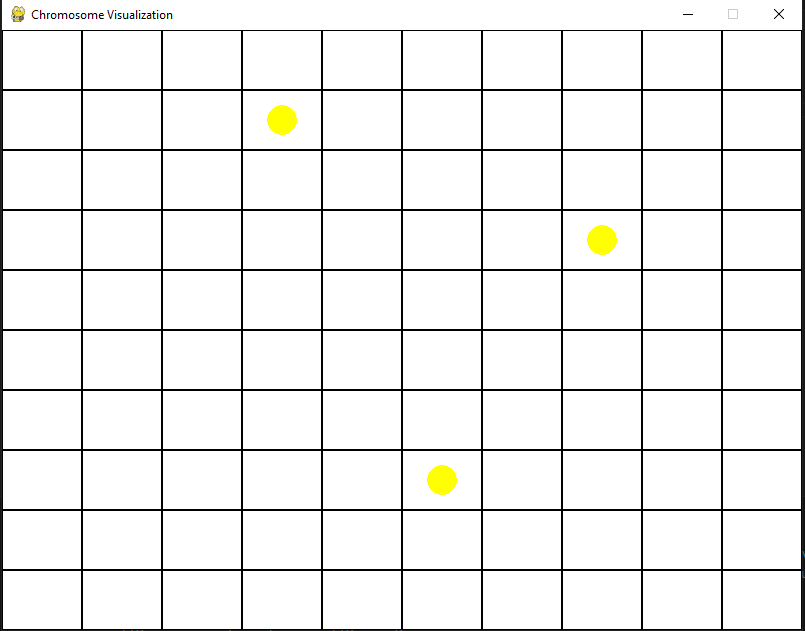
\includegraphics[width=0.5\textwidth]{chromosone.PNG}}
    \label{chromosone}
\end{figure}

The chromosome is created using the chromosome function, which requires a Room object in addition to the width and height of the room and produces a collection of light placements inside the room dimensions at random to be used as a starting point for the genetic algorithm's optimization process.
\\
Overall, chromosome structure is important in the genetic algorithm because it offers a possible solution to the optimization problem and is subject to crossover, mutation, and selection during the evolutionary process.

\subsection{Fitness Function}
The fitness function is a statistic used in computational intelligence problems to assess the quality of a solution. The fitness function, in this scenario, is intended to evaluate the effectiveness of a chromosome, which represents a candidate solution to the optimization problem of maximizing the number of lighted tiles in a room while minimizing the number of lights put on the room's ceiling.\\
\\
The fitness function requires a Room object and a list of light positions as input. It generates a fitness value indicating how effectively the given chromosome handles the optimization problem.\\

The fitness value is computed as the weighted sum of two objectives:
\begin{itemize}
    \item Maximization of illuminated tiles.
    \item Minimization of lights in the chromosome.\\
\end{itemize}

The fitness function begins by lighting up the tiles in the room by first using the $Room.light.tiles()$ method which lights up the corresponding lights with regard to the chromosome given. After which $Room.num.lit.tiles()$ method is called which counts the number of lighted tiles, this method takes in all the factors such as obstacles, sunlight, and shadows. The number of lighted tiles reflects one of the fitness function's objectives, which we wish to maximize.\\
\\
The fitness function then computes the number of lights employed in the chromosome by lengthening the list of light spots. The number of lights indicates the other fitness function objective that we wish to minimize.\\

The fitness function employs a   weighted sum to integrate these two objectives into a single fitness value. Each objective's weight, w, shows its relative importance. If w is close to $1$, the number of lighted tiles becomes the most important criterion in judging fitness. If w is close to zero, the number of lights in the chromosome will take precedence. A value of w of $0.5$ indicates that both objectives are equally important.

\begin{table}[htbp]
    \caption{Fitness Values for 5 possible solutions}
    \begin{center}
        \begin{tabular}{|p{3.0cm}|p{1.0cm}|p{1.5cm}|p{1.0cm}|}
            \hline
            \textbf{Chromosome} & \textbf{\textit{Num Lit Tiles}} & \textbf{\textit{Num Lights}} & \textbf{\textit{Fitness}} \\
            \hline
            [(0, 2), (2, 3), (3, 1)] & 100 & 3 & 48.5 \\
            \hline
            [(1, 0), (2, 2), (4, 1), (0, 4)] & 98 & 4 & 46.0 \\
            \hline
            [(0, 3), (2, 1)] & 95 & 2 & 45.5 \\
            \hline
            [(3, 2), (2, 3), (1, 1), (0, 2), (2, 0)] & 99 & 5 & 47 \\
            \hline
            [(1, 0), (3, 3), (0, 4)] & 97 & 3 & 45.5 \\
            \hline
        \end{tabular}
        \label{fitnes_table}
    \end{center}
\end{table}


The fitness value is then computed as:
\begin{center}
 $Fitness = w * num.lit.tiles - (1 - w) * num.lights$    
\end{center}
This results in a greater fitness value for chromosomes that light up more tiles while using fewer lights.
\\\\
Table \ref{fitnes_table} shows the fitness values for five possible solutions. The chromosome with the highest fitness value is the first one, $[(0, 2), (2, 3), (3, 1)]$, which has a fitness value of $48.5$. This chromosome uses only three lights to illuminate $100$ tiles in the room. $[(3, 2), (2, 3), (1, 1), (0, 2), (2, 0)]$ is the second-best chromosome, which illuminates $99$ tiles with $5$ lights and has a fitness value of $47$. The first chromosome has the highest fitness value since it can illuminate the most tiles with the fewest lights, which is the goal of the optimization task.\\
\\
After calculating the fitness value, the function restores the room to its starting state and returns the fitness value and the tile grid as a tuple. The tile grid is later used for visualizing the lighted tiles and checking for fitness function flaws.
\subsection{Crossover}
The crossover function is a genetic operator used in genetic algorithms to integrate genetic information from two parent chromosomes, often to produce offspring with novel genetic combinations. In our lighting optimization challenge, as mentioned the chromosomes represent potential light placements in a given room.

Given two parent chromosomes, parent1, and parent2, the crossover function chooses two genes at random from the parents to represent potential light locations.\\

The function then finds the minimum and maximum of the two selected genes to decide the start and end genes for breeding.
\begin{itemize}
    \item $Child1$ is generated by combining the genes from $parent1$ between the start and finish genes.
    \item $Child2$ is formed by combining the genes from $parent2$ that are not already present in child1.\\
\end{itemize}

Finally, the function joins child1 and child2 to form the final offspring chromosome, which represents a new set of possible light places in the room. The function returns the offspring chromosome as its output.
\begin{table}[h!]
  \centering
  \caption{Parent Information and Crossover Points}
  \begin{tabular}{|p{1.5cm}|p{1.5cm}|p{0.5cm}|p{0.5cm}|p{0.5cm}|p{0.5cm}|}
    \hline
    Parent1 & Parent2 & Gene1 & Gene2 & Start Gene & End Gene \\
    \hline
    [(1, 2), (3, 4), (5, 6)] & [(2, 4), (6, 1), (8, 2)] & 1 & 2 & 1 & 2 \\
    \hline
  \end{tabular}
  \label{parent-info}
\end{table}
\\ In \ref{parent-info} the crossover is performed between the $2$ parents. Two random genes are chosen from the parents, and the start and end genes for crossing are based on the values of the selected genes. So, in this case, $Gene1$ is $1$ and $Gene2$ is $2$, consequently, the start gene is $1$ and the end gene is $2$.
\begin{table}[h!]
  \centering
    \caption{Offspring}

  \begin{tabular}{|c|c|c|}
    \hline
    Child1 & Child2 & Offspring \\
    \hline
    [(1, 2), (6, 1)] & [(3, 4), (8, 2)] & [(1, 2), (6, 1), (3, 4), (8, 2)] \\
    \hline
  \end{tabular}
  \label{offspring}
\end{table}
\\ In \ref{offspring} it is shown Child1 is the first offspring formed by taking genes from Parent1 from start.gene to end.gene. $Child1$ is $[(1, 2), (6, 1)]$ in the aforementioned situation as it inherits the genes $(1, 2)$ and $(6, 1)$ from Parent1. Child2 is produced by taking genes from Parent2 that were not present in Child1. So, $Child2$ is $[(3, 4), (8, 2)]$ since it contains the genes $(3, 4)$ and $(8, 2)$ from Parent2.\\\\
By concatenating Child1 and Child2, we get the final offspring $[(1, 2), (6, 1), (3, 4), (8, 2)]$.



\subsection{Mutation}
The mutation function accepts an individual chromosome (list of possible light locations) and mutates light positioning by swapping two spots from the list of light positions.\\ 
\begin{itemize}
    \item It chooses two random indices to exchange in each chromosome.
    \item  At the specified indices, swaps the two chromosomes.
    \item The mutated chromosome is returned.\\ 
\end{itemize}

To give an example, let's assume we have an individual $[ (1, 2), (3, 4), (5, 6), (7, 8), (9, 10) ]$. Upon applying our mutate function it will randomly generate $2$ indexes to swap positions, let's assume these to be $2$ and $4$. The function will then swap the chromosome at these indexes and will return the mutated chromosome, which is $[ (1, 2), (9, 10), (5, 6), (7, 8), (3, 4) ]$.\\


This function contributes to the diversification of the population of viable solutions and keeps the algorithm from becoming stuck in a local minimum.
\subsection{Parent and Survivor Selection}
The selection process is a crucial component of any evolutionary algorithm in the context of an optimization problem. It is in responsibility for choosing the most optimal individuals (or "parents") from the existing population to establish the population's future generation. Truncation selection and tournament selection are two prevalent methods of selection.
\\\\
Truncation selection entails choosing the best performers in the population and employing them as parents to develop the next generation. Typically, the number of individuals chosen for breeding is a predetermined percentage of the population size. This strategy is straightforward to apply and frequently leads to rapid convergence to a satisfactory solution, particularly in situations with a relatively smooth fitness landscape.
\\\\
Tournament selection entails selecting a subset of individuals at random from the population and then selecting the best-performing individual from that subset as the parent for the following generation. This procedure is repeated until the desired number of parents is chosen. This strategy is more stochastic than truncation selection and can help to maintain genetic diversity within the population, which is useful in more difficult optimization problems with a rough fitness landscape.
\\\\
In the current optimization problem, truncation selection and tournament selection were employed for parent and survivor selection, respectively, because they produced the best results. When truncation selection is used, only the fittest individuals are chosen as parents for the following generation, whereas tournament selection allows for a broader spectrum of survivors and is able to prevent premature convergence.

\section{Experiments and Results}
We ran our Evolutionary Algorithm for every hour of the day which yielded
different results depending on the \textit{Sun's} altitude at that moment. We
fixed the number of generations to 100 with a population size of 30, and the
other \textit{Evolutionary Algorithm} parameters were also kept constant. We
ran our experiments with varying positions of the window and arbitrary obstacles
in the room.

\subsection{North facing Window}
``Fig.~\ref{n_hourly}'' a fixed window at the north side of the room, we ran our experiments for
24 hours with an interval of 3 hours between each run. In the obtained graph we can see that the
number of lights decreases as the sun's altitude increases. This is because the sunlight is able to
light up the room and the number of lights required to light up the room decreases. The number of
lights then decreases as the sun sets and the room gets darker. There is some inconsistency in the
graph but that is because of the arbitrary obstacles and the number of generations. ``Table.~\ref{n_hourly_table}'' shows the light positions for each hour of the day. The fitness value for each hour is also shown in the table.

\begin{figure}[htbp]
    \centerline{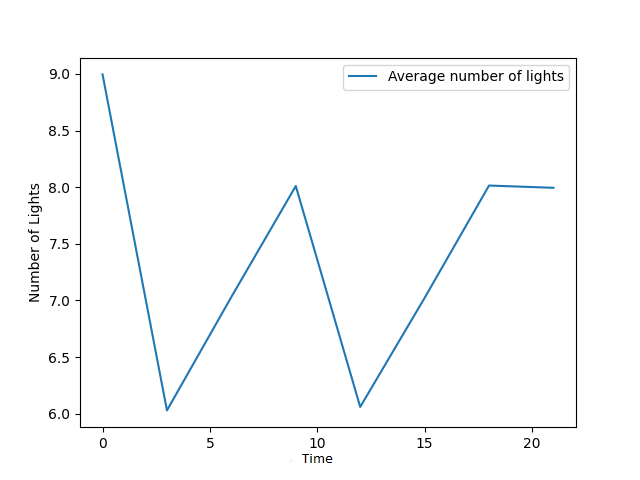
\includegraphics[width=0.5\textwidth]{n_hourly.png}}
    \caption{Average number of lights in a room with a North facing window}
    \label{n_hourly}
\end{figure}

\begin{table}[htbp]
    \caption{Light Positions for North facing window}
    \begin{center}
        \begin{tabular}{|c|c|c|c|}
            \hline
            \textbf{Time} & \textbf{\textit{Light Positions ($x, y$)}}               & \textbf{\textit{n}} & \textbf{\textit{Fitness}} \\
            \hline
            12 am         & [(9, 8), (6, 1), (1, 8), (4, 5), (1, 0),                 & 7                   & 46.5                      \\
                          & (0, 0), (9, 1)]                                          &                     &                           \\
            \hline
            3 am          & [(8, 1), (6, 8), (0, 0), (0, 1), (5, 4),                 & 7                   & 46.0                      \\
                          & (1, 5), (3, 0)]                                          &                     &                           \\
            \hline
            6 am          & [(8, 8), (4, 7), (5, 4), (4, 5), (0, 8),                 & 10                  & 45.0                      \\
                          & (8, 1), (0, 3), (0, 1), (5, 0), (1, 0)]                  &                     &                           \\
            \hline
            9 am          & [(9, 9), (8, 1), (6, 0), (5, 8), (2, 2),                 & 7                   & 46.5                      \\
                          & (0, 7), (1, 0)]                                          &                     &                           \\
            \hline
            12 pm         & [(8, 1), (6, 8), (5, 9), (5, 3), (1, 0),                 & 8                   & 46.0                      \\
                          & (5, 5), (5, 7), (0, 6)]                                  &                     &                           \\
            \hline
            3 pm          & [(9, 4), (7, 0), (1, 4), (5, 5), (3, 4)]                 & 5                   & 45.5                      \\
            \hline
            6 pm          & [(9, 9), (7, 4), (7, 1), (1, 6), (5, 6),                 & 7                   & 46.0                      \\
                          & (4, 2), (1, 1)]                                          &                     &                           \\
            \hline
            9 pm          & [(8, 9), (3, 7), (5, 8), (2, 0), (3, 2), & 10                  & 44.5                      \\
                          &  (5, 4), (0, 0), (3, 9), (1, 5), (7, 4)]                                  &                     &                           \\
            \hline
        \end{tabular}
        \label{n_hourly_table}
    \end{center}
\end{table}

\subsection{East facing Window}
Similarly, for an \textit{East facing window} we got the following ``Fig.~\ref{n_hourly_obsless_e}'' graph.
In the obtained graph we can see that the number of lights is minimum during the morning hours as the \textit{Sun}
rises from the east and lights up the room. The number of lights then increases as the \textit{Sun's} altitude increases
and sets in the west.
\begin{figure}[htbp]
    \centerline{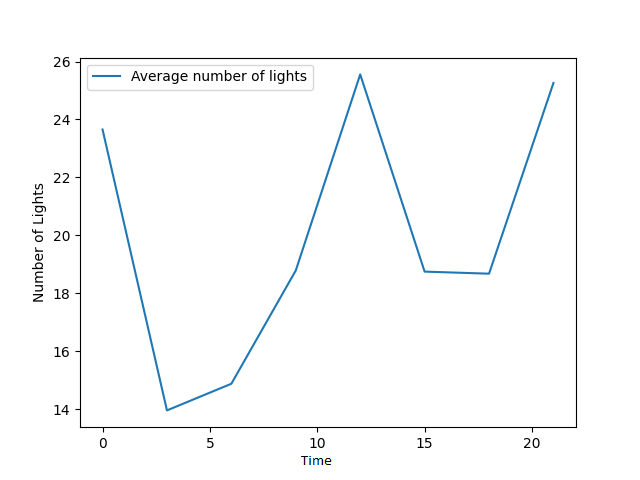
\includegraphics[width=0.5\textwidth]{n_hourly_obsless_e.png}}
    \caption{Average number of lights in a room with an East facing window}
    \label{n_hourly_obsless_e}
\end{figure}

\subsection{West facing Window}
``Fig.~\ref{n_hourly_obsless_w}'' shows the results for a \textit{West facing
    window}. In the obtained graph we can see that the number of lights is
minimum during the evening hours as the \textit{Sun} sets in the west and lights
up the room. The number of lights then increases as the \textit{Sun} sets and
the room gets darker.
\begin{figure}[htbp]
    \centerline{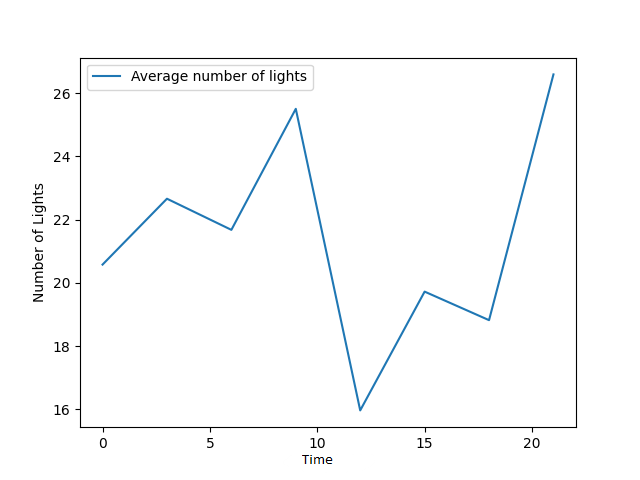
\includegraphics[width=0.5\textwidth]{n_hourly_obsless_w2.png}}
    \caption{Average number of lights in a room with a West facing window}
    \label{n_hourly_obsless_w}
\end{figure}

\subsection{Visualization}
``Fig.~\ref{visualization}'' shows the visualization of the room with a window facing North and obstacles toward the east side of the room. The white tiles show that they are lit whereas the dark grey tiles are a region that is not lit. Moreover, the regions having lighter shades of gray, show tiles that are partially lit according to the light intensity they are receiving, considering all the factors of our optimization problem. However, our visualization requires more enhancement to show our results efficiently.
\begin{figure}[htbp]
    \centerline{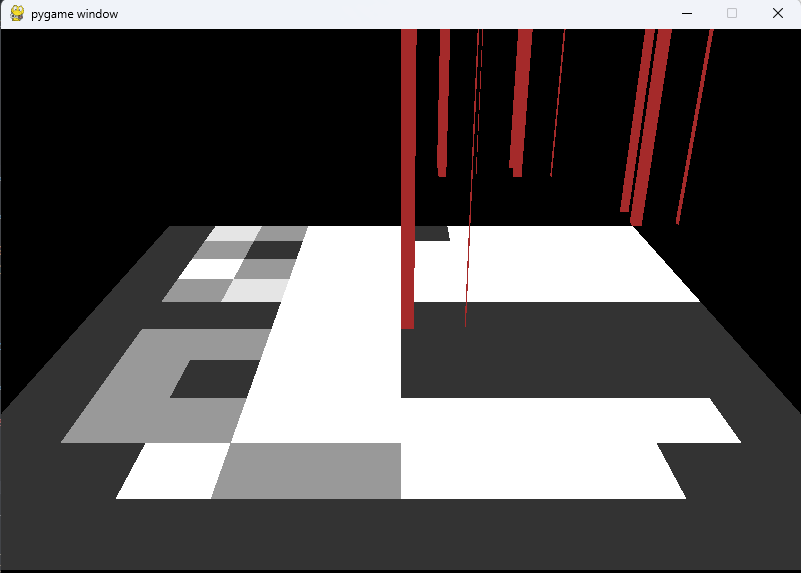
\includegraphics[width=0.5\textwidth]{pygame.png}}
    \caption{Visualization of the room with a North facing window and obstacles}
    \label{visualization}
\end{figure}

\section{Conclusion}
In this paper we have proposed a method to optimize the number of lights in a
room. We have used an \textit{Evolutionary Algorithm} to find the optimal
positions for the lights depending on the position of the window and the angle
of the \textit{Sun}. We have also taken into account the obstacles in the room
which may block the light from reaching certain parts of the room. We have
performed experiments for different positions of the window and different
obstacles in the room. We have also performed experiments for different times of
the day. We observed that the number of lights is minimum when the window is
facing the \textit{Sun} and the number of lights increases as the window faces
away from the \textit{Sun} which agrees with logic.

\section{Future Work}
This paper is currently limited in terms of the number of experiments
performed. We plan to perform more experiments in order to get more accurate
results. We also plan to use a more accurate model for the \textit{Sun's}
position which takes into account the \textit{Earth's} elliptical orbit by
using the \textit{Sun's} azimuth angle as well. We also plan to use a more
accurate model for the \textit{Sun's} intensity which can help us illuminate
the room more accurately, and find more precise positions for the lights. Moreover, for our visualization, we aim to use more profound tools that can correctly display our results, such as Blender.


\begin{thebibliography}{00}
    \bibitem{icict_2019} Saleha R. Aiman K. Sami M. Optical Illumination of rooms using Genetic
    Algorithm. 2019
    \bibitem{occupant} Anca D. Galasiu and Jennifer A. Veitch. “Occupant preferences and satis-
faction with the luminous environment and control systems in Daylit Of-
fices: A Literature Review”. In: Energy and Buildings 38.7 (2006), pp. 728–
742. doi: 10.1016/j.enbuild.2006.03.001.
    \bibitem{solar} Richard Perez et al. “Modeling daylight availability and irradiance com-
ponents from direct and global irradiance”. In: Solar Energy 44.5 (1990),
pp. 271–289. doi: 10.1016/0038-092x(90)90055-h.
    \bibitem{ephem} \textit{Ephem}. [Online]. Available: https://rhodesmill.org/pyephem/index.html. [Accessed: 10- May- 2023].
    \bibitem{ref9}\label{ref9} Goldberg, D. E. (1989). Genetic Algorithms in Search, Optimization, and Machine Learning. Reading: Addison-Wesley.
\end{thebibliography}

\end{document}